\chapter{Fravælgelse af gestik-par}
\label{app:TestresultaterFravaelgelse}
%
Hat
%
\section{Fravælgelse af gestik-par til pause og start}
\label{app:TestresultaterPauseDaarlig} 
%
I følgende afsnit analyseres hvilke af de syv semaforiske gestik-par testpersonerne fravælger samt hvorfor testpersonerne netop fravælger disse gestik-par. På baggrund af analysen bør det være muligt at udpege, hvilke semaforiske gestikker, der i hvert fald ikke skal knyttes til hverken pause eller start. Analysen bygger på testpersonerne respons til spørgsmålet: \textit{Hvilken gestik kan du mindst lide? og hvorfor?}, hvor testpersonernes samlede data er vedlagt i \autoref{app:NoterValgAfGestikker}.
%
\begin{figure}[H]
	\centering
	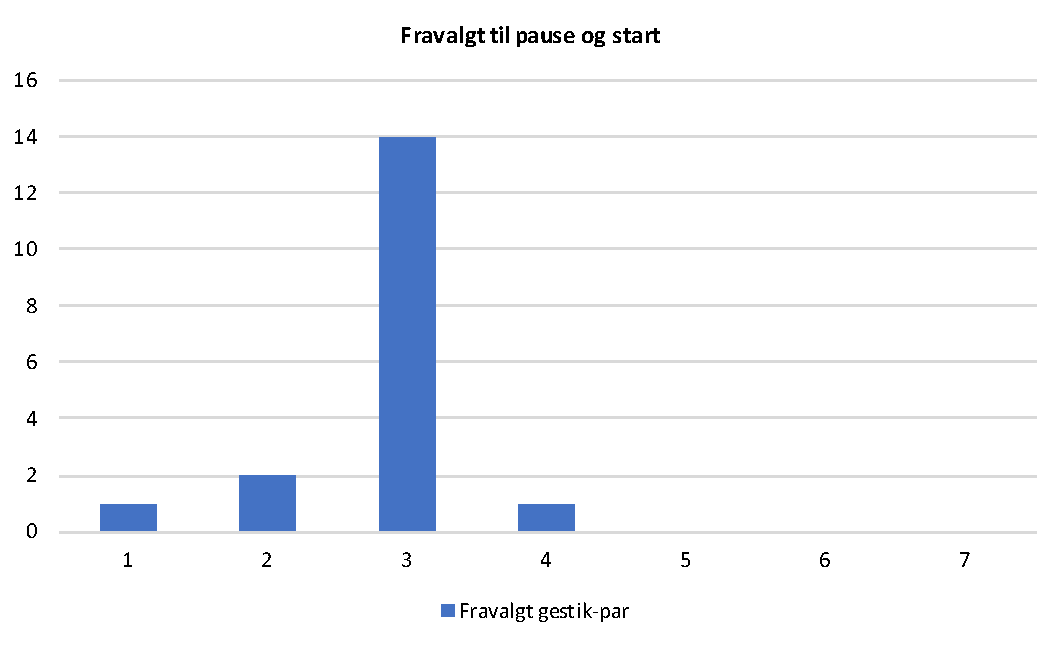
\includegraphics[resolution=300,width=0.9\textwidth]{Test1/DatabehandlingGrafer/FravalgtPause}
	\caption{Barplot over hvilke gestik-par testpersonerne fravælger i forbindelse med pause og start.}
	\label{fig:DaarligstGestikPause}
\end{figure}
\noindent
% 
På \autoref{fig:DaarligstGestikPause} fremgår det hvilke gestik-par de 18 testpersoner fravælger i forbindelse med at skulle pause og starte musikken. Det fremgår tydeligt at gestik-par 3 er det gestik-par, som flest testpersoner fravælger i forhold til de tre andre gestik-par, der ellers er repræsenteret på \autoref{fig:DaarligstGestikPause}. Gestik-par 3 illustreres på \autoref{fig:GestikPar3Pause}. Derudover fravælges gestik-par 1 af én testperson, testperson 13, fordi testpersonen forbinder det med at række en hånd i vejret. Testperson 1 og testperson 8 fravælger gestik-par 2 på baggrund af bevægelsesmængden, hvor begge testpersoner giver udtryk for, at der er for meget unødvendig bevægelse. Årsagen til at testperson 5 fravælger gestik-par 4 skyldes at testpersonen generelt ikke bryder sig om at pege. Gestik-par 4 illustreres på \autoref{fig:GestikPar4Pause}. I og med at testperson 5 både kommenterer at gestik-par 4 er aggressiv og at det vil føles mærkeligt at stå derhjemme og pege, så tyder det på at testpersonen oplever gestik-par 4 som værende social uacceptabel. 
%
\begin{figure}[H]
	\centering
	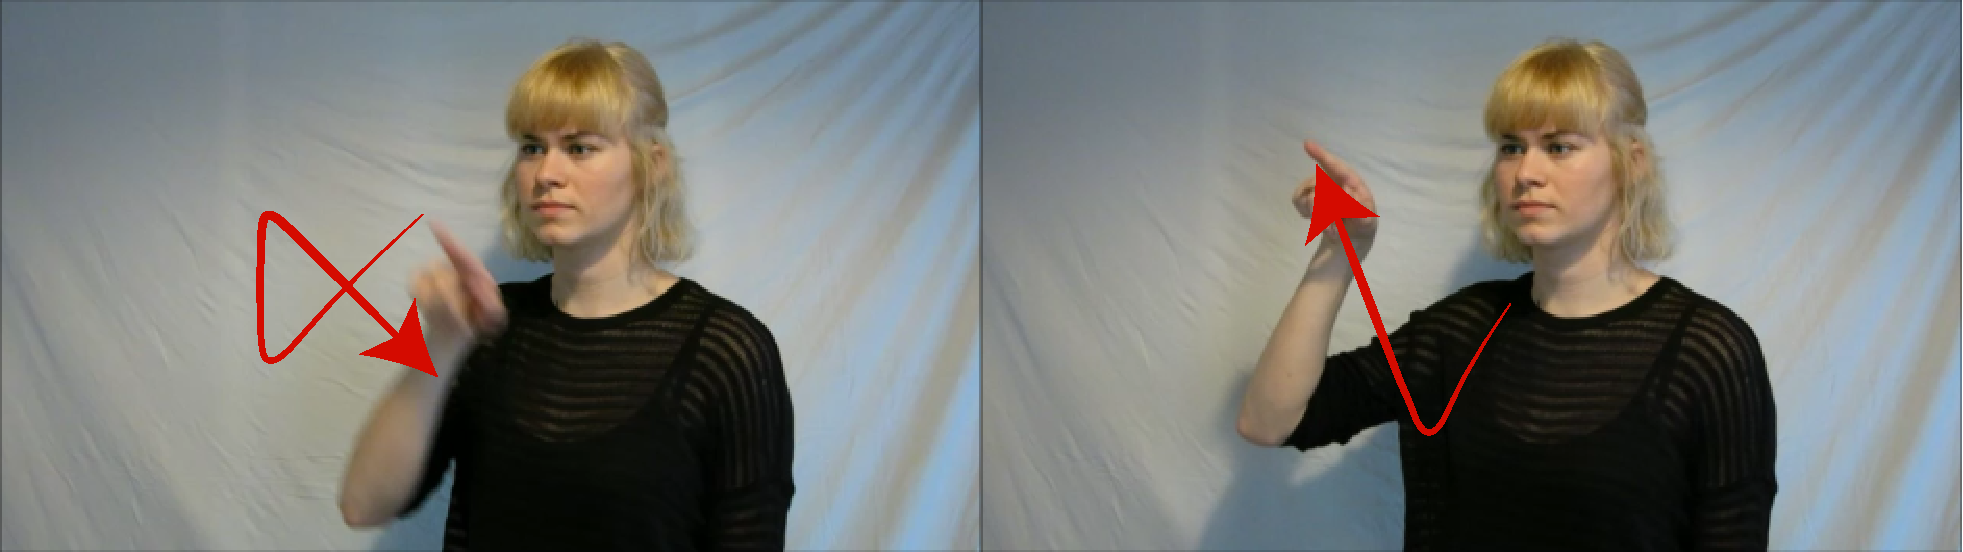
\includegraphics[resolution=300,width=0.9\textwidth]{Test1/Gestik-par/Gestik3_Pause}
	\caption{Illustration af gestik-par 3; kryds til pause og flueben til start.}
	\label{fig:GestikPar3Pause}
\end{figure}
\noindent
% 
De resterende 14 testpersoner fravælger alle gestik-par 3, illustreret på \autoref{fig:GestikPar3Pause}. De to største årsager til at gestik-parret fravælges skyldes kompleksiteten i bevægelsen og at det simpelthen er for besværeligt at udføre. I forhold til bevægelsen giver flere testpersoner udtryk for at den, foruden at være kompleks, enten er for underlig, testperson 3, for mærkelig, testperson 4, for lang og akavet, testperson 7 og for indviklet, testperson 12. I tillæg kommenterer testperson 17, at det bliver en større øvelse at skulle pause og starte musikken, og så vil der gå lang tid før musikken rent faktisk bliver sat på pause. Derudover giver testperson 14 og testperson 15 udtryk for, at det ikke er sikkert, at de kan huske hvordan bevægelsen er, når den så skal udføres. I tillæg giver testperson 14 udtryk for ikke, at ville vide hvordan musikken pauses eller startes igen. Testperson 9 giver udtryk for lignede bekymringer omkring hvordan musikken sættes på pause og startes igen.

Af de 18 testpersoner, der har deltaget i testen, er der kun to; testperson 8 og testperson 13, som har inkluderet gestik-par 3 i deres top tre rangering. Begge testpersoner tildeler gestik-par 3 en første plads, lige indtil at testperson 8 til sidst skal gengive de fortrukne gestikker og indtil at testperson 13 skal lave en forbedring, hvorefter gestik-parret, i begge tilfælde, tildeles en anden plads. Årsagerne til at testperson 8 har inkluderet gestik-par 3 blandt de tre bedste er dels fordi den er unik, speciel og sjov, men den gav også en fornemmelse af at det ikke bare var en knap, der blev trykket på. Testperson 13 inkluderer derimod gestik-par 3 fordi det ikke er en typisk bevægelse at udføre og dermed vil testpersonen ikke komme til at pause musikken ved et uheld.\blankline
%
For at afgøre hvilke af de syv gestik-par, der skal fravælges, er det nødvendigt at sammenholde hvilke gestikker testpersonerne fravælger med de gestikker, som indgår i testpersonernes top tre rangering. Der opstilles derfor en tabel over de fire fravalgte gestik-par og hvordan de indgår i testpersonernes rangering.
%
\begin{table}[H]
	\centering
	\begin{tabular}{ | p{2.4cm} | p{2.4cm} | p{2.4cm} | p{2.4cm} | p{2.4cm} |}
	\hline
		 & Gestik-par 1 & Gestik-par 2 & Gestik-par 3 & Gestik-par 4 \\ \hline
		1. Plads & 8 & 1 & 0 & 0\\ \hline
		2. Plads & 3 & 3 & 2 & 1\\ \hline
		3. Plads & 2 & 0 & 0 & 2\\ \hline
	\end{tabular}
	\caption{Oversigt over hvor ofte og hvor de fire fravalgte gestikker indgår i testpersonernes top tre rangering.}
	\label{tab:FravalgteTopTrePause}
\end{table}
\noindent
%
På baggrund af \autoref{tab:FravalgteTopTrePause} tyder det på, at det eneste gestik-par, der flerstemmigt kan ekskluderes, er gestik-par 3, dels fordi parret kun indgår i to testpersoners top tre og dels fordi 14 testpersoner har fravalgt det. Derudover er gestik-par 4, illustreret på \autoref{fig:GestikPar4Pause}, kun inkluderet tre gange i testpersonernes samlede top tre rangering, jævnfør \autoref{tab:FravalgteTopTrePause}, og da gestik-parret ydermere er fravalgt, blandt andet på baggrund af det er socialt uacceptabelt, vurderes det at der ligeledes er belæg for, at ekskludere gestik-par 4 fra fremtidige undersøgelser.  
%
\begin{figure}[H]
	\centering
	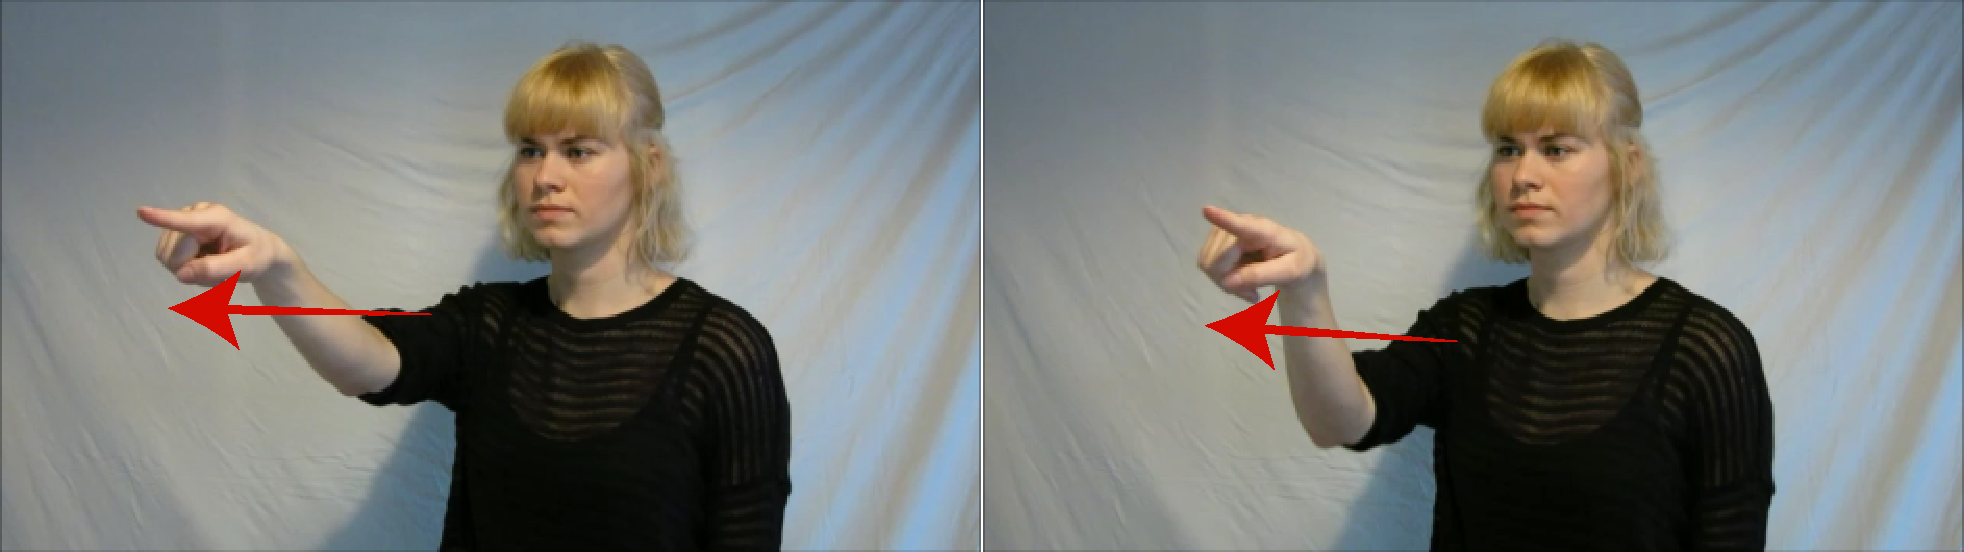
\includegraphics[resolution=300,width=0.9\textwidth]{Test1/Gestik-par/Gestik4_Pause}
	\caption{Illustration af gestik-par 4; pegefingeren peger og trykker i luften hen mod musikanlægget for henholdvis pause og start.}
	\label{fig:GestikPar4Pause}
\end{figure}
\noindent
% 
I forhold til gestik-par 2 så tyder det på, at gestik-parret kun indgår i testperson 3's top tre rangering, fordi testpersonen forbinder de andre forslag med mute og testpersonen giver ydermere udtryk for, at det ikke giver meningen at lave et dynamisk stop-tegn, svarende til gestik-par 2. Gestik-par 2 illustreres på \autoref{fig:GestikPar2Pause}. Der skal dog tages forbehold for at testperson 3, ud fra testpersonens respons, virker forvirret og selvmodsigende. Ifølge testperson 7 bliver gestik-par 2 inkluderet i top tre rangeringen, fordi det virkede lige til og at det er det testpersonen forbinder med et stop-tegn. Årsagen til at testperson 10 inkluderer gestik-par 2 kan ikke direkte udledes af testpersonens udsagn, men generelt har testpersonen valgt gestikker, som var nemme at huske og med en lav risiko for at gestikken enten gengives med en forkert bevægelse eller udføres ved et uheld. Den eneste testperson, som har tildelt gestik-par 2 en første plads er testperson 12 og årsagen til det skyldes at testpersonen som udgangspunkt ville have valgt gestik-par 1, som den bedste og forbedret gestikken ved at tilføje bevægelsen, der gengives i gestik-par 2, jævnfør \autoref{fig:GestikPar2Pause}. Men derudover giver testperson 12 udtryk for, at være fascineret af gestik-par 5, hvorfor det vurderes at det måske også vil tilfredsstille testpersonen, hvis gestik-par 5 blev valgt. 
%
\begin{figure}[H]
	\centering
	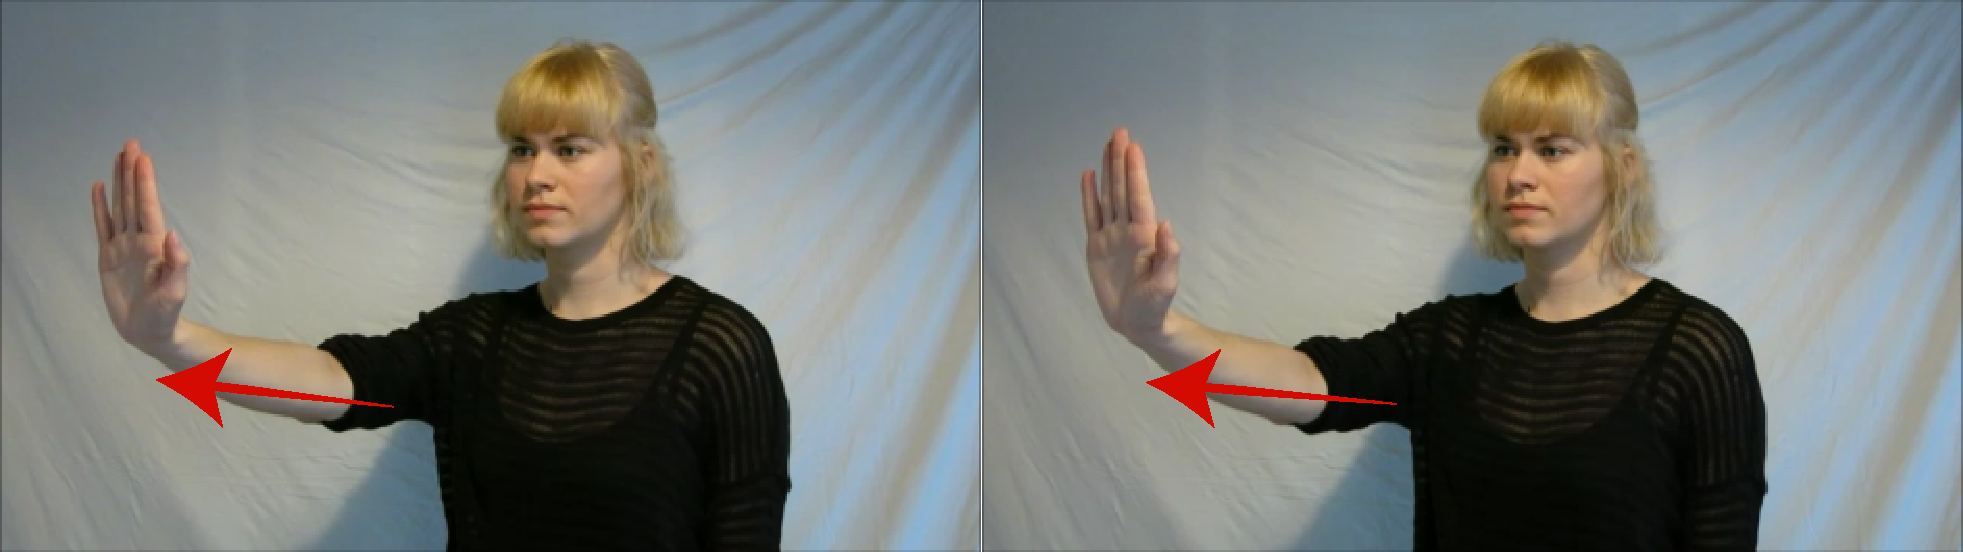
\includegraphics[resolution=300,width=0.9\textwidth]{Test1/Gestik-par/Gestik2_Pause}
	\caption{Illustration af gestik-par 2; dynamisk vertikal hånd, der starter ved brystet og ender i en udstrakt horisontal arm.}
	\label{fig:GestikPar2Pause}
\end{figure}
\noindent
% 
Argumenterne for at fravælge gestik-par 2 kan, blandt andet, sammenholdes med responsen fra både testperson 1 og testperson 8, som begge vurderer, at der er unødvendigt meget bevægelse i. Derudover blev der i \fullref{Socialaccept}, blandt andet, inddraget en undersøgelse hvori det blev konkluderet at testpersonerne følte sig mest komfortable når afstanden mellem dem og selve interaktionen var lille, hvilket ligeledes understøtter argumenterne for at fravælge gestik-par 2. Selvom fokus for denne del af undersøgelsen ikke vedrører social accept, så tyder det på, at desto tættere på kroppen gestikkerne udføres, desto større er sandsynligheden for, at de indgår i testpersonernes top tre. Så baseret på de foregående argumenter og fordi gestik-par 2 kræver en bevægelse langt fra kroppen, i forhold til de andre forslag samt at gestik-parret kun fremgår fire gange i testpersonernes samlede top tre, jævnfør \autoref{tab:FravalgteTopTrePause}, så vælges det at ekskludere gestik-par 2 fra fremtidige undersøgelser. 
%
\section{Fravælgelse af gestik-par til at skifte musiknummer}
\label{app:TestresultaterSkiftDaarlig}
%
I følgende afsnit analyseres hvilke af de syv semaforiske gestik-par testpersonerne fravælger samt hvorfor testpersonerne netop fravælger disse gestik-par. På baggrund af analysen bør det være muligt at udpege hvilke semaforiske gestikker, der i hvert fald ikke skal knyttes til at skifte musiknummer. Analysen bygger på testpersonerne respons til spørgsmålet: \textit{Hvilken gestik kan du mindst lide? og hvorfor?}, hvor testpersonernes samlede data er vedlagt i \autoref{app:NoterValgAfGestikker}.
%
\begin{figure}[H]
	\centering
	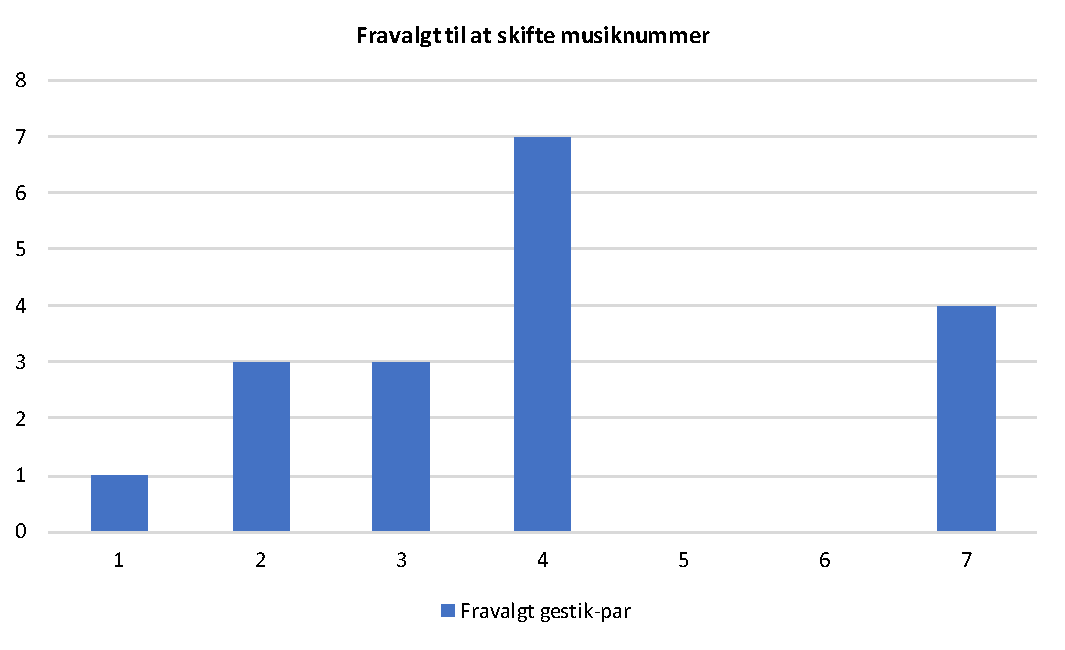
\includegraphics[resolution=300,width=0.9\textwidth]{Test1/DatabehandlingGrafer/FravalgtSkift}
	\caption{Barplot over hvilke gestik-par testpersonerne fravælger i forbindelse med at skifte musiknummer frem og tilbage.}
	\label{fig:DaarligstGestikSkift}
\end{figure}
\noindent
%
På \autoref{fig:DaarligstGestikSkift} fremgår det, hvilke gestik-par de 18 testpersoner fravælger i forbindelse med at skifte musiknummer. Det fremgår tydeligt at gestik-par 4 er det gestik-par, som flest testpersoner fravælger i forhold til de resterende gestik-par repræsenteret på \autoref{fig:DaarligstGestikSkift}. Gestik-par 4 illustreres på \autoref{fig:GestikPar4Skift}. Derudover fravælges gestik-par 7 næstflest gange, mens gestik-par 2 og gestik-par 3 begge fravælges tre gange og gestik-par 1 fravælges en enkelt gang. Årsagen til at testperson 14 har valgt gestik-par 1, som værende den testpersonen mindst kan lide, begrundes med at testpersonen forestiller sig, at det er en bevægelse testpersonen vil komme til at gengive gentagende gange foran sit musikanlæg eller under en samtale. Testperson 1, testperson 5 og testperson 16 har alle valgt gestik-par 2, som værende den de mindst kan lide, fordi gestikken er modsat af, hvad de forventer er frem og tilbage. At gestik-par 3 fravælges begrunder testperson 3, testperson 11 og testperson 13 med, at hvis der skulle peges i en retning så skulle det være med pegefingeren og ikke tommelfingeren, da det er en akavet bevægelse og fordi gestikken er statisk. I den forbindelse giver testperson 5 udtryk for heller ikke at bryder sig om hverken gestik-par 3 eller gestik-par 7, netop fordi de er statiske.
%
\begin{figure}[H]
	\centering
	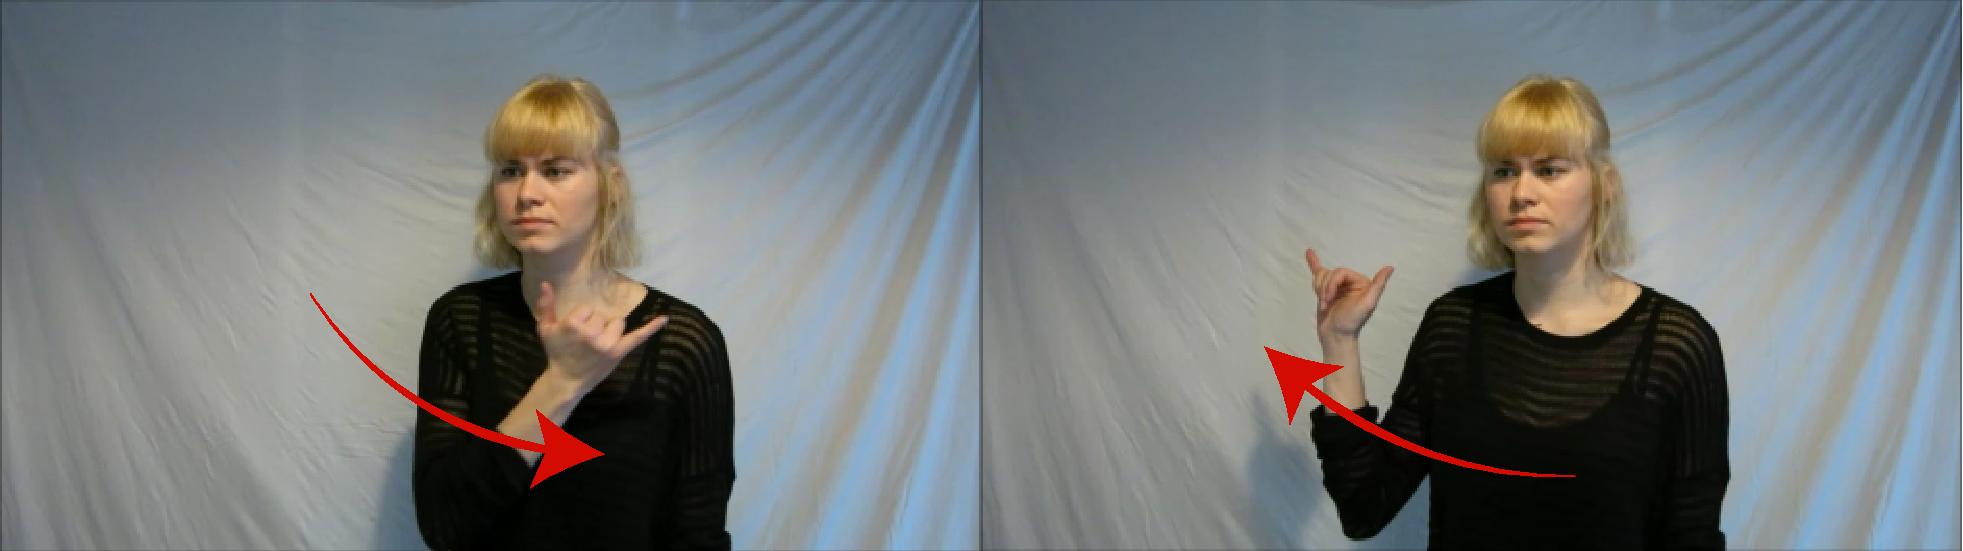
\includegraphics[resolution=300,width=0.9\textwidth]{Test1/Gestik-par/Gestik4_SkiftSang}
	\caption{Illustration af gestik-par 4; swipe-bevægelse fra højre mod venstre med tommel- og lillefinger strakt, mens de andre fingre bøjes for at skifte til det næste musiknummer og swipe fra venstre mod højre for at skifte til det forrige musiknummer.}
	\label{fig:GestikPar4Skift}
\end{figure}
\noindent
%
Der er forskellige årsager til at syv testpersoner fravælger gestik-par 4. Testperson 4 og testperson 6 fravælger gestikken, fordi den er mærkelig, hvor testperson 4 forbinder det med at skulle tage telefonen. Testperson 8 forstår ikke, hvorfor det er lige præcis er det håndtegn, der skal bruges. Testperson 10 oplever ikke at gestikken bringer noget nyt, men snarere at det er en besværlig version af gestik-par 5. I forhold til håndtegnet i gestik-par 4, så kommenterer testperson 12 at det er unaturligt at gøre noget med lillefingere, testperson 7 kommenterer dels, at det er en stor armbevægelse og dels, at det er et sjovt håndtegn, som vil blive glemt, hvis det ikke bliver brugt. I tillæg kommenterer testperson 18 ligeledes, at det er en unaturlig gestik, som vil blive glemt. Dog pointerer testpersonen, at det er en effektiv gestik i og med at den ikke vil blive lavet ved en fejl.
%
\begin{figure}[H]
	\centering
	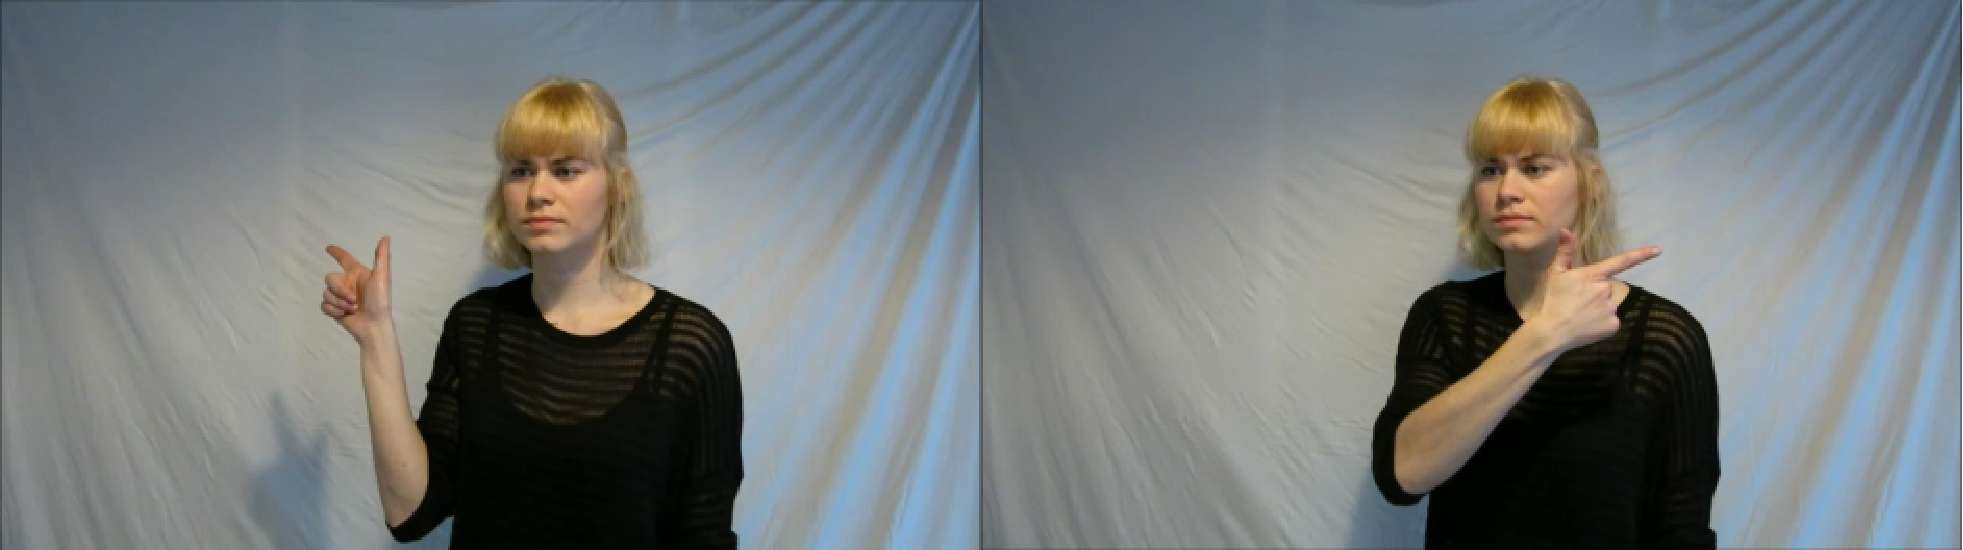
\includegraphics[resolution=300,width=0.9\textwidth]{Test1/Gestik-par/Gestik7_SkiftSang}
	\caption{Illustration af gestik-par 7; peg med tommel- og pegefinger til højre eller venstre for henholdvist at skifte til næste eller forrige musiknummer.}
	\label{fig:GestikPar7Skift}
\end{figure}
\noindent
% 
Årsagen til at gestik-par 7 fravælges skyldes ifølge testperson 2, testperson 9 og testperson 17, dels at den virkede mærkelig, dels at den ikke blev opfattet og dels at den minder om en pistol. Gestik-par 7 illustreres på \autoref{fig:GestikPar7Skift}. Ligesom gestik-par 3 blandt andet blev fravalgt, fordi den er statisk, så fravælger testperson 15 af samme årsag gestik-par 7 og i tillæg påpeger at det er et enkelt tegn.\blankline
%
For at afgøre hvilke af de syv gestik-par, der skal fravælges, er det nødvendigt at sammenholde hvilke gestikker testpersonerne fravælger med de gestikker, som indgår i testpersonernes top tre rangering. Der opstilles derfor en tabel over de fem fravalgte gestik-par og hvordan de indgår i testpersonernes rangering.    
%
\begin{table}[H]
	\centering
	\begin{tabular}{ | p{1.5cm} | p{2.1cm} | p{2.1cm} | p{2.1cm} | p{2.1cm} | p{2.1cm} |}
	\hline
		 & Gestik-par 1 & Gestik-par 2 & Gestik-par 3 & Gestik-par 4 & Gestik-par 7 \\ \hline
		1. Plads & 10 & 3 & 1 & 0 & 0\\ \hline
		2. Plads & 2 & 3 & 3 & 0 & 1\\ \hline
		3. Plads & 0 & 0 & 7 & 5 & 2\\ \hline
	\end{tabular}
	\caption{Oversigt over hvor ofte og hvor de fem fravalgte gestikker indgår i testpersonernes top tre rangering.}
	\label{tab:FravalgteTopTreSkift}
\end{table}
\noindent
%
På baggrund af \autoref{tab:FravalgteTopTreSkift} sammenholdt med \autoref{fig:DaarligstGestikSkift}, tyder det på at gestik-par 4 og gestik-par 7 kan ekskluderes fra fremtidige undersøgelser. Det skyldes at selvom gestik-par 4 indgår fem gange i testpersonernes top tre, så fravælges gestik-parret af syv testpersoner. Derudover tyder det på, at de fem testpersoner, som har inkluderet gestik-par 4 i deres top tre, har gjort det på baggrund af bevægelsen snarre end kombinationen af både håndtegnet og bevægelsen. Gestik-par 7 ekskluderes, da gestik-parret kun indgår tre gange i testpersonernes samlede top tre og da den derudover fravælges af fire testpersoner. 
%
\begin{figure}[H]
	\centering
	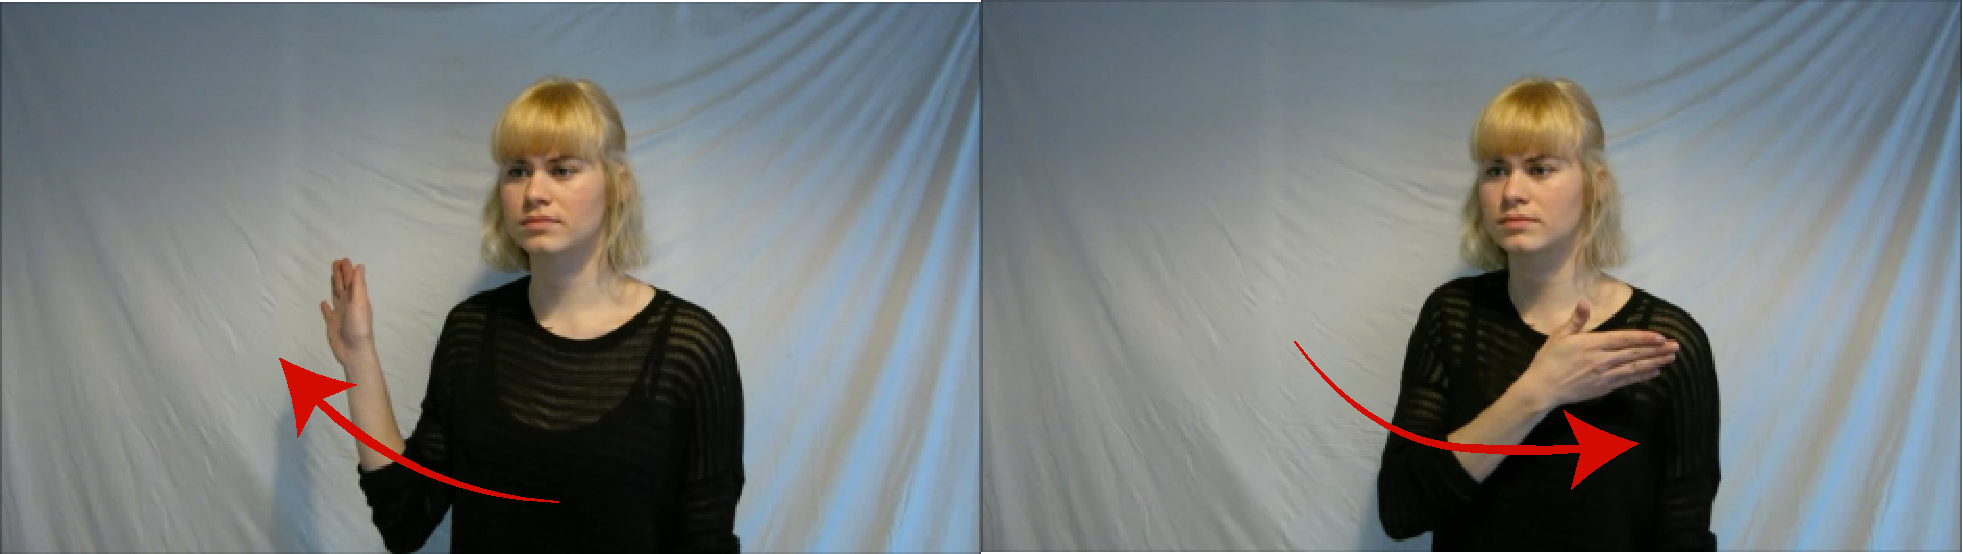
\includegraphics[resolution=300,width=0.9\textwidth]{Test1/Gestik-par/Gestik2_SkiftSang}
	\caption{Illustration af gestik-par 2; swipe-bevægelse fra venstre mod højre for at skifte til det næste musiknummer og swipe fra højre mod venstre for at skifte til det forrige musiknummer.}
	\label{fig:GestikPar2Skift}
\end{figure}
\noindent
%
De tre testpersoner, som fravælger gestik-par 2, gør det formentligt fordi de har en mental model af, at hvis der swipes fra højre mod venstre så afspilles det næste musiknummer i playlisten, modsat hvis der swipes fra venstre mod højre så afspilles det forrige musiknummer. Gestik-par 2 illustreres på \autoref{fig:GestikPar2Skift}. De tre testpersoner, der har tildelt gestik-par 2 en første plads, har formentligt den modsatte mentale model af hvilken swipe-bevægelse, der skal udføres for at skifte til det næste musiknummer. For at det kan afgøres hvorvidt gestik-par 2 skal ekskluderes eller ej, så er det nødvendigt at undersøge nærmere hvilke gestik-par de seks testpersoner, som har inkluderet gestik-par 2 i deres top tre, ellers har inkluderet. 
%
\begin{table}[H]
	\centering
	\begin{tabular}{ | p{3cm} | p{3cm} | p{3cm} | p{3cm} |}
	\hline
		 & 1. Plads & 2. Plads & 3. Plads \\ \hline
		Testperson 4 & Gestik-par 2 & Gestik-par 5 & Gestik-par 3 \\ \hline
		Testperson 17 & Gestik-par 2 & Gestik-par 3 & Gestik-par 4 \\ \hline
		Testperson 18 & Gestik-par 2 & Gestik-par 1 & Gestik-par 3 \\ \hline
		Testperson 8 & Gestik-par 3 & Gestik-par 2 & Gestik-par 7 \\ \hline
		Testperson 12 & Gestik-par 1 & Gestik-par 2 & Gestik-par 5\\ \hline
		Testperson 15 & Gestik-par 1 & Gestik-par 2 & Gestik-par 5 \\ \hline
	\end{tabular}
	\caption{Oversigt over de seks testpersoner, som enten har tildelt gestik-par 2 en første eller en anden plads i top tre, samt hvilke gestik-par de ellers har inkluderet.}
	\label{tab:GestikPar2ITopTre}
\end{table}
\noindent
%
Sammenholdes testperson 4's top tre rangering med testpersonens udsagn og bevægelser i videooptagelserne, så tyder det på at denne testperson har en mental model af, at hvis der swipes fra højre mod venstre så afspilles det forrige musiknummer kontra et swipe fra venstre mod højre, som vil afspille det næste musiknummer. Testpersonen kommenterer ydermere, at gestik-par 5 også vil fungere såfremt retning var omvendt, svarende til hvad der gengives i gestik-par 2, som illustreres på \autoref{fig:GestikPar2Skift}. Testperson 17, som ligeledes har tildelt gestik-par 2 en første plads, udfører også de korrekte bevægelser i forhold til testpersonens egne kommenterer. Dog opstår der usikkerhed, når testpersonen afslutningsvist skal gengive sine fortrukne gestikker. Efter en diskusion med testlederen konkluderer testperson 17 dog at det stadig er gestik-par 2, der er bedst. Selvom testperson 18 virker sikker i sit valg om, at det er gestik-par 2, der er det bedste gestik-par, så gengiver testpersonen rent faktisk bevægelserne fra gestik-par 1, dog med venstre hånd. Når testpersonen i tillæg forklarer hvad swipe-bevægelserne gør i forhold til at skifte til det forrige eller det næste musiknummer, relaterer det sig ligeledes til gestik-par 1. Det er derfor ikke til at vide hvorfor testpersonen har rangeret gestik-par 2 højere end gestik-par 1. Det tyder derfor på at den eneste testperson, der med sikkerhed vil vælge swipe-bevægelserne i gestik-par 2, er testperson 4. 

Rettes fokus mod de tre testpersoner, som har rangeret gestik-par 2 på en anden plads, så tyder det på at de to testpersoner, som har tildelt gestik-par 1 en første plads, hovedsageligt har inkluderet gestik-par 2 på grund af bevægelsen. Dog kommenterer testperson 15, at gestik-par 2 er modsat af hvad testpersonen finder logisk. Derudover pointerer testperson 12, at det var svært at adskille gestik-par 1 fra gestik-par 2. Testperson 8 har derimod rangeret gestik-par 2 mellem de to statiske gestik-par og når testpersonen gengiver bevægelserne i gestik-par 2 så stemmer det både overens med testpersons udsagn samt hvordan gestik-parret er designet. Det tyder derfor på at testpersonen rent faktisk har valgt gestik-par 2 fordi det stemmer overens med testpersonens mentale model.\blankline 
%
Ud af de seks testpersoner er det kun testperson 4 og testperson 8, der rent faktisk giver entydigt udtryk for at deres mentale model af gestik-par 2 stemmer overens både med deres bevægelser og deres udsagn. Derudover er der i Bang $\&$ Olufsen's produkter desuden truffet en designbeslutning om, at en swipe-bevægelse fra højre mod venstre resulterer i at det er det næste musiknummer afspilles, da dette stemmer overens med at trække det næste musiknummer frem. På baggrund af den foregående analyse og da det ikke ønskes at gå i mod Bang $\&$ Olufsen's designvalg, vurderes det derfor at der er tilstrækkeligt belæg for at ekskludere gestik-par 2. 

På baggrund af foregående analyse forefindes der ikke et tilstrækkeligt belæg for hverken at ekskludere gestik-par 1 eller gestik-par 3, hvorfor disse vil undersøges nærmere. 
%
\section{Fravælgelse af gestik-par til at skrue op og ned for musikken}
\label{app:TestresultaterVolumenDaarlig}
%
I følgende afsnit analyseres hvilke af de ni semaforiske gestik-par testpersonerne fravælger samt hvorfor testpersonerne netop fravælger disse gestik-par. På baggrund af analysen bør det være muligt at udpege hvilke semaforiske gestikker, der i hvert fald ikke skal knyttes til at skrue op og ned for musikken. Analysen bygger på testpersonerne respons til spørgsmålet: \textit{Hvilken gestik kan du mindst lide? og hvorfor?}, hvor testpersonernes samlede data er vedlagt i \autoref{app:NoterValgAfGestikker}.
%
\begin{figure}[H]
	\centering
	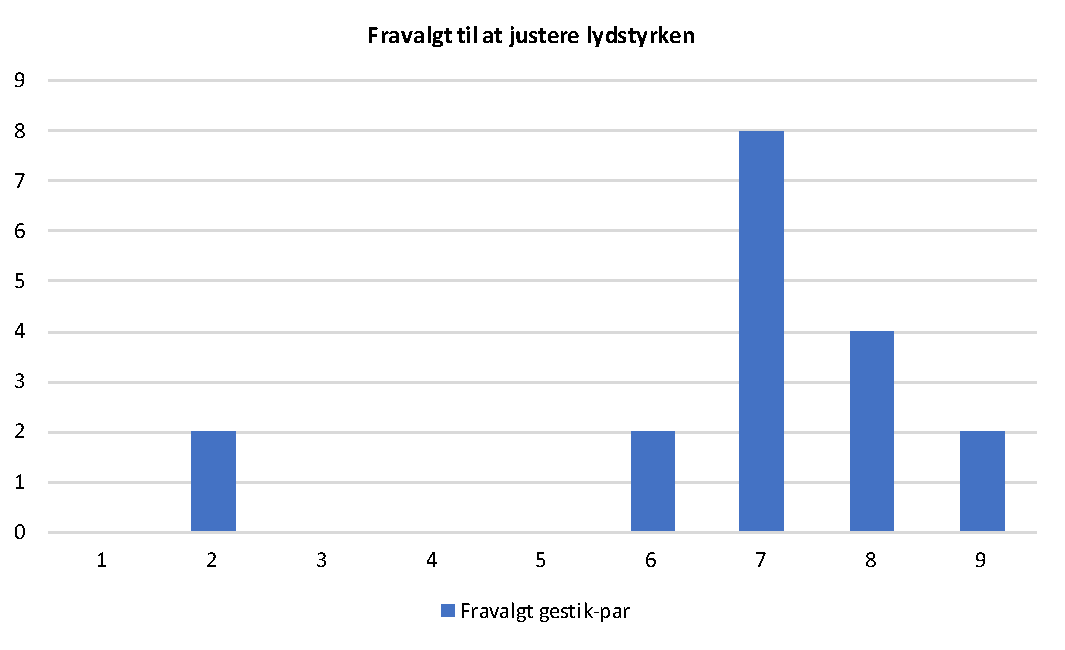
\includegraphics[resolution=300,width=0.9\textwidth]{Test1/DatabehandlingGrafer/FravalgtVolumen}
	\caption{Barplot over hvilke gestik-par testpersonerne fravælger i forbindelse med at skrue op og ned for musikken.}
	\label{fig:DaarligstGestikVolumen}
\end{figure}
\noindent
%
På \autoref{fig:DaarligstGestikVolumen} fremgår det, hvilke gestik-par de 18 testpersoner fravælger i forbindelse med at skrue op og ned for musikken. Det fremgår tydeligt at testpersonerne hyppigst fravælger gestik-par 7, da gestik-parret i alt er fravalgt otte gange, og ikke indgår på en eneste top tre rangering, jævnfør \autoref{tab:GestikParITopTreVolumen}. Gestik-par 7 illustreres på \autoref{fig:GestikPar7Volumen}. Årsagen til at gestik-par 7 fravælges varierer mellem de otte testpersonerne, som har valgt gestik-parret. Testperson 2 har svært ved at vurdere hvilken vej der er op og hvilken vej der er ned. Ifølge testperson 3 er gestik-par 7 underlig og derudover så giver det ikke mening. At gestik-parret ikke giver mening pointere testperson 15 også og tilføjer, at det er en mellemting mellem gestik-par 5 og gestik-par 6. Testperson 4 fravælger gestikken, fordi den er mærkelig, hvilket også er en af årsagerne til at testperson 11 fravælger gestik-parret. Derudover kommenterer testperson 11, at det kræver koncentration at gengive en bue, hvilket er en del af bevægelsen. Da formålet med at anvende semaforiske gestikker til at interagere med Bang $\&$ Olufsen's fremtidige musikanlæg, blandt andet er for at interaktionen på sigt kan foregå i den perifere opmærksomhed, så er det ikke hensigtsmæssigt at gestikkerne kræver mere koncentration end andre løsninger. Derudover påpeger testperson 10, at gestik-par 7 er væsentligt mindre intuitiv end de andre forslag og dertil er det svært at vurdere den nødvendige bevægelsesmængde for at skrue op og ned. Ifølge testperson 6 så er gestik-par 7 det par, som skiller sig mest ud i forhold til de andre forslag, hvilket er årsagen til at parret fravælges. Testperson 14's respons afviger fra de andre testpersoners, i det at testperson 14 fravælger gestik-par 7, fordi testpersonen anser det som værende en meget naturlig bevægelse, som testpersonen giver udtryk for at ville komme til at lave ubevidst.
%
\begin{figure}[H]
	\centering
	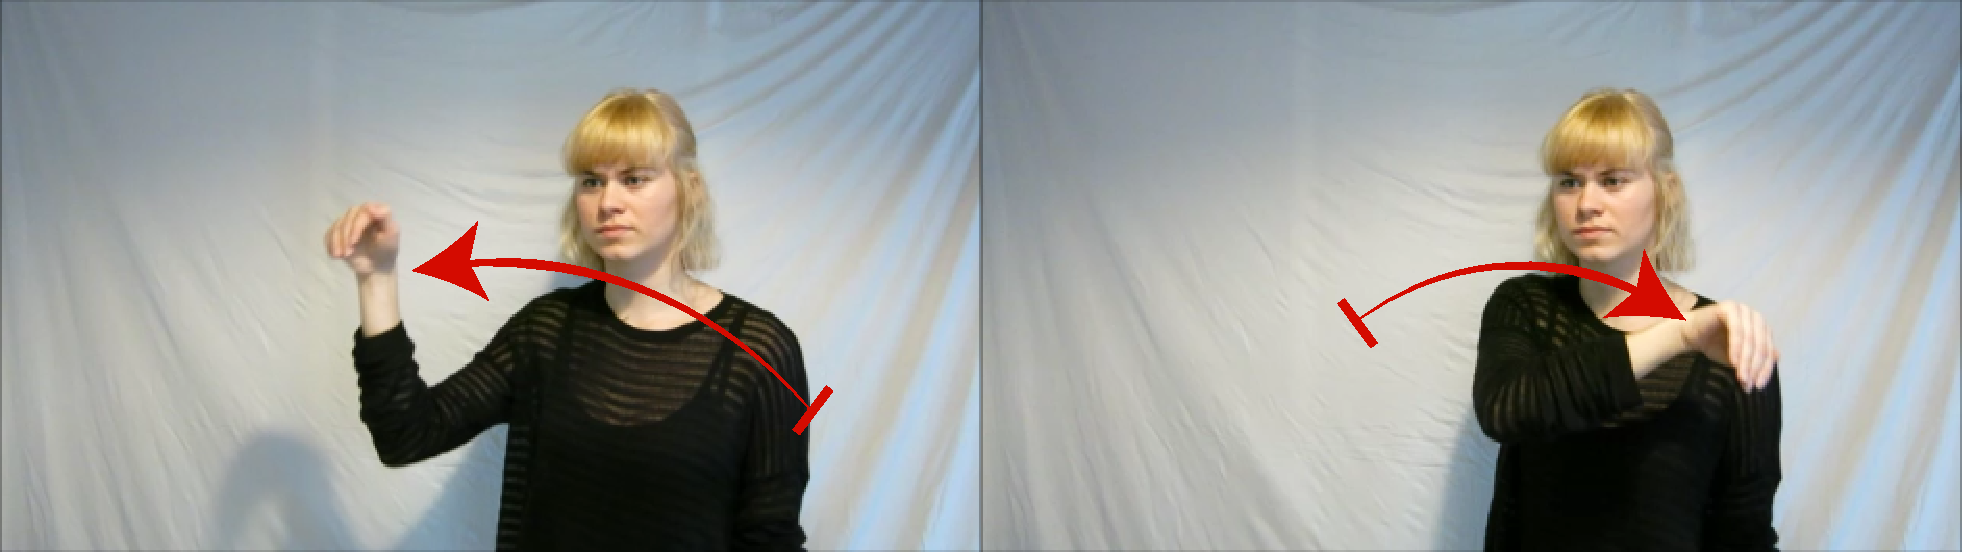
\includegraphics[resolution=300,width=0.9\textwidth]{Test1/Gestik-par/Gestik7_Volumen}
	\caption{Illustration af gestik-par 7; krum hånd bevæges i en bue fra venstre mod højre for at skrue op og fra højre mod venstre for at skrue ned, svarende til hvordan det gøres på A9, \parencite{WEB:BeoplayA9}.}
	\label{fig:GestikPar7Volumen}
\end{figure}
\noindent
%
Selvom gestik-par 7 blev inkluderet som et forsøg på at overfører gestikken, der anvendes til at skrue op og ned på en A9, \parencite{WEB:BeoplayA9}, til en semaforisk gestik, så er gestik-par 7 det par, som oftes fravælges og som ikke indgår i nogen af testpersonernes top tre, hvorfor gestik-parret ekskluderes.
%
\begin{figure}[H]
	\centering
	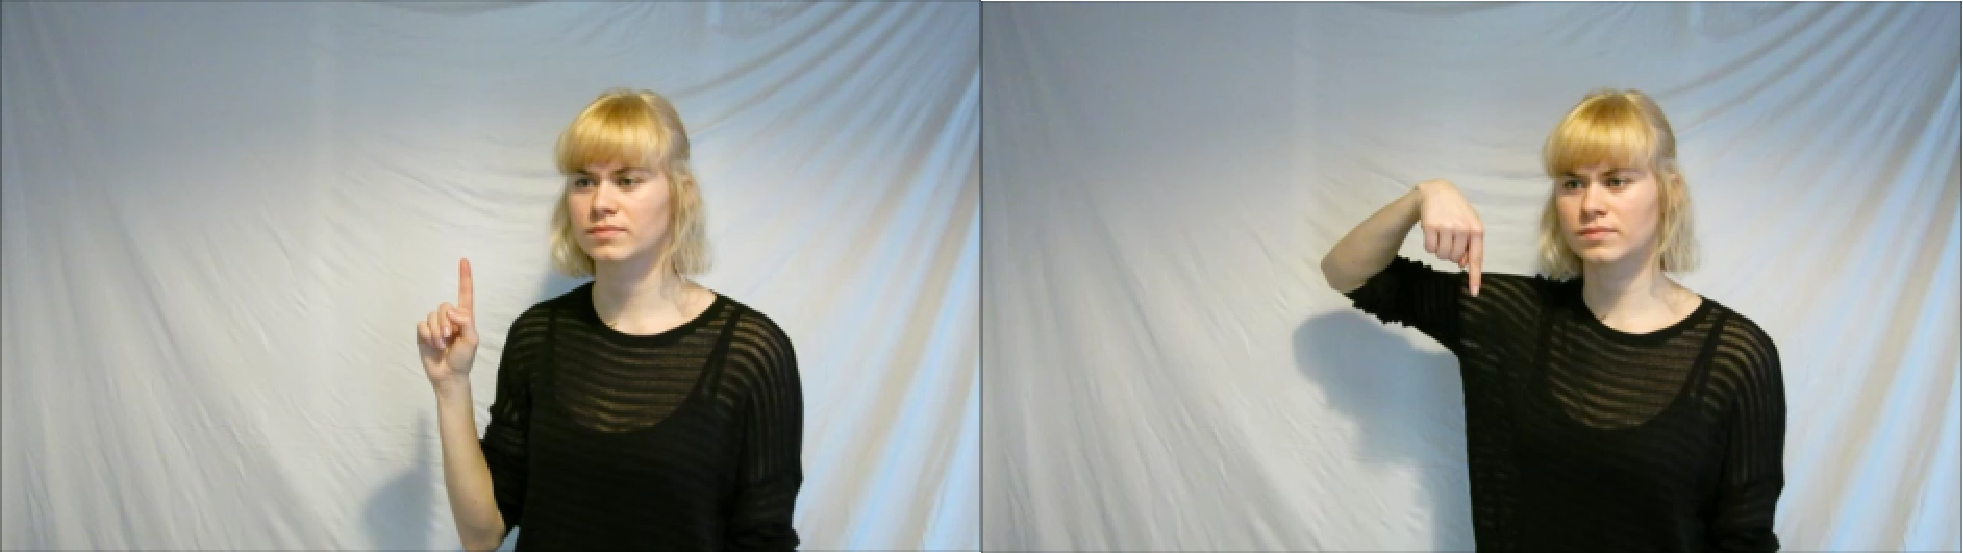
\includegraphics[resolution=300,width=0.9\textwidth]{Test1/Gestik-par/Gestik8_Volumen}
	\caption{Illustration af gestik-par 8; pegefingeren peger op for at skrue op og peger ned for at skrue ned.}
	\label{fig:GestikPar8Volumen}
\end{figure}
\noindent
%
To ud af de fire testpersoner, som fravælger gestik-par 8, giver udtryk for at det er besværligt at pege nedad. Gestik-par 8 illustreres på \autoref{fig:GestikPar8Volumen}. Den ene af de to, testperson 18, giver stærkt udtryk for, at det er både besværligt og ubehagligt at pege nedad samt at have sin arm i den position, jævnfør \autoref{fig:GestikPar8Volumen}. Den anden af de to testpersoner, testperson 9, giver udtryk for at det besværligt at gengive og det er underligt at pege nedad. Derudover pointerer testperson 9, at det er svært at kontrollere, hvor meget der enten skal skrues og eller ned, hvilket også er årsagen til at testperson 5 fravælger gestik-par 8; der er ingen mulighed for at kontrollere hvor meget der skrues op. Den sidste af de fire testpersoner, testperson 13, fravælger gestik-par 8 fordi der mangler bevægelse og fordi det er noget testpersonen godt kunne forestille sig komme til at gøre ved et uheld. \blankline 
%
Der er to forskellige årsager til hvorfor gestik-par 2 fravælges af testperson 12 og testperson 16. Testperson 12 fravælger gestik-par 2, fordi testpersonen ikke bryder sig om cirkelbevægelsen, selvom testpersonen pointerer at det burde virke naturligt og det egentlig er sådan der normaltvist skrues op på et musikanlæg. Det skal dog pointeres at testperson 12 ikke endegyldigt fastslår, at det er gestik-par 2, der er værst, da testpersonen egentlig heller ikke bryder sig om gestik-par 1. Grunden til at det fremgår, at testperson 12 har valgt gestik-par 2 som værende dårligst, er på baggrund af de bevægelser, der opstår når testpersonen skal forklare hvorfor der vælges som der gør. I dette tilfælde stemte bevægelsen overens med bevægelsen i gestik-par 2. Årsagen til at gestik-par 2 fravælges af testperson 16, er fordi bevægelsen er modsat af hvad testpersonen forventer. Det skal dog pointeres at der ved gestik-par 2 skrues op for musikken ved at dreje hånden med uret og skrues ned ved at dreje hånden mod uret, hvilket er det testpersonen egentlig forventer. Det tyder derfor på at testperson 16 har misforstået videooptagelsen af gestik-par 2. Testlederen spørger derfor ind til hvordan gestik-par 2 kunne gøres bedre, hvor testperson 16 først og fremmest foreslår, at bevægelsen foregår i den rigtige retning og derudover foreslår testpersonen, at gestikken skulle være mere ligesom gestik-par 1, hvor testpersonen referer til armens position. 

Gestik-par 6 fravælges af testperson 9 fordi det vil være svært, at gengive bevægelsen med et barn på armen, hvilket også gør sig gældende for gestik-par 5. Gestik-par 6 illustreres på \autoref{fig:GestikPar6Volumen}. Testperson 17 fravælger gestik-par 6 fordi det er ulogisk at lave den bevægelse i forbindelse med musik og derudover virker det mærkeligt at begge hænder skal være involveret. 

Ifølge testperson 7 så fravælges gestik-par 9 fordi den ikke tillader kontrol over hvor meget der skrues op og ned, hvorimod testperson 8 fravælger gestik-par 9 fordi testpersonen vil have det akavet med at lave den bevægelse.\blankline
%
For at afgøre hvilke af de ni gestik-par, foruden gestik-par 7, som allerede er ekskluderet, der skal fravælges, er det nødvendigt at sammenholde hvilke gestikker testpersonerne fravælger med de gestikker, som indgår i testpersonernes top tre rangering. Der opstilles derfor en tabel over de fem fravalgte gestik-par og hvordan de indgår i testpersonernes rangering.    
%
\begin{table}[H]
	\centering
	\begin{tabular}{ | p{1.5cm} | p{2.1cm} | p{2.1cm} | p{2.1cm} | p{2.1cm} | p{2.1cm} |}
	\hline
		 & Gestik-par 2 & Gestik-par 6 & Gestik-par 7 & Gestik-par 8 & Gestik-par 9 \\ \hline
		1. Plads & 4 & 1 & 0 & 0 & 2\\ \hline
		2. Plads & 2 & 2 & 0 & 0 & 1\\ \hline
		3. Plads & 3 & 1 & 0 & 2 & 3\\ \hline
	\end{tabular}
	\caption{Oversigt over hvor ofte og hvor de fem fravalgte gestikker indgår i testpersonernes top tre rangering.}
	\label{tab:FravalgteTopTreVolumen}
\end{table}
\noindent
%
På baggrund af \autoref{tab:FravalgteTopTreVolumen} hvor gestik-par 9 fremgår seks gange i testpersonernes top tre rangering sammenholdt med \autoref{fig:DaarligstGestikVolumen} samt testpersonernes begrundelser for hvorfor de fravælger gestik-par 9, vurderes det at der er ikke er belæg for at ekskludere gestik-par 9. Det vurderes ydermere, at der ikke forefindes tilstrækkeligt belæg for at ekskludere gestik-par 2, for selvom det ikke kan antages med sikkerhed, at testperson 16 ville have udpeget et andet gestik-par, i tilfælde af at testpersonen ikke havde misforstået bevægelsesretningen, så tyder det på, at det godt kunne være tilfældet. I så fald er det kun testperson 12, som har givet udtryk for at en cirkulærbevægelse ikke foretrækkes. Da det heller ikke entydigt kan konkluderes, hvorvidt testperson 12 mindst kan lide gestik-par 2 i forhold til gestik-par 1 og da gestik-par 2 sammenlagt indgår ni gange i testpersonernes top tre, jævnfør \autoref{tab:FravalgteTopTreVolumen}, vurderes det at der ikke er belæg for at ekskludere gestik-par 2 .
%
Baseret på \autoref{tab:FravalgteTopTreVolumen} hvor gestik-par 8 kun indgår to gange i testpersonernes samlede top tre rangering sammenholdt med \autoref{fig:DaarligstGestikVolumen} samt testpersonernes begrundelser for, hvorfor de fravælger gestik-par 8, vurderes det at der er belæg for at ekskludere gestik-par 8. 
%
\begin{figure}[H]
	\centering
	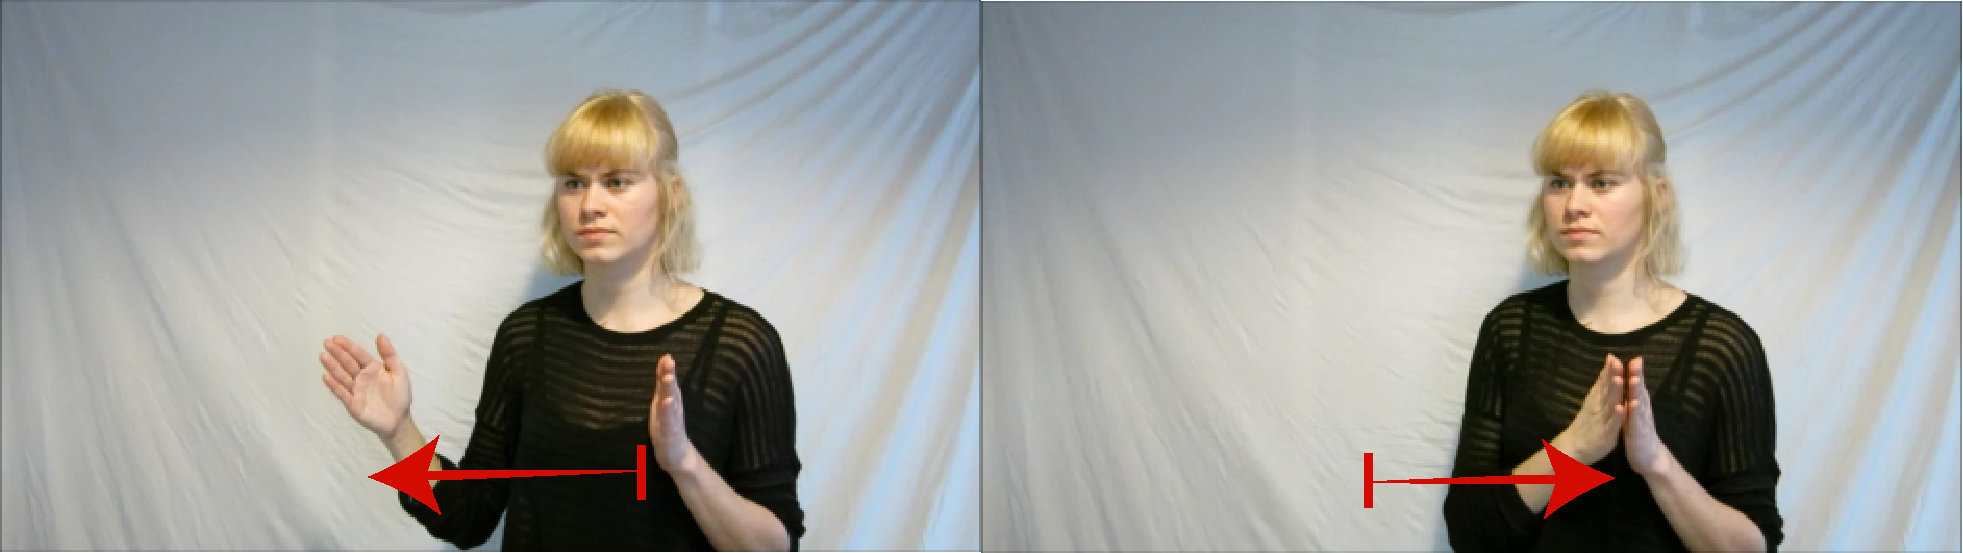
\includegraphics[resolution=300,width=0.9\textwidth]{Test1/Gestik-par/Gestik6_Volumen}
	\caption{Illustration af gestik-par 6; vertikal ikke-dominant hånd holdes stationær, ems den dominante hånd ligeledes holdes vertikal og bevægelser sig væk fra den ikke-dominante hånd i en horisontal bevægelse for at skrue op og for at skrue ned bevæges den dominante hånd mod den ikke-dominante hånd.}
	\label{fig:GestikPar6Volumen}
\end{figure}
\noindent
% 
For at have belæg for at ekskludere gestik-par 6 er det nødvendigt at inkludere hvad testpersonerne, som har rangeret gestik-par 6 i deres top tre, har kommenteret. Ifølge testperson 1 så indgår gestik-par 6 på en anden plads dels fordi den følger et princip om noget, der er større eller mindre, jævnfør \autoref{fig:GestikPar6Volumen}, og dels fordi bevægelsen er naturlig. Det tyder på at testperson 14 rangerer gestikker alt efter hvad der føles akavede og unaturligt i frygt for at komme til at lave gestikkerne ved et uheld, hvilket er årsagen til at testperson 14 har tildelt gestik-par 6 en anden plads. Testperson 2 forklarer at årsagen til at gestik-par 6 rangeres på en tredje plads, er fordi den minder om gestik-par 4 og gestik-par 5 bare sidelæns, men at det ikke giver lige så meget mening, som de to andre. Baseret på testperson 5's udsagn tyder det på at årsagen til at gestik-par 6 tildeles en første plads er fordi testpersonen ønsker at have fuld kontrol over, hvor meget der skrues op og ned, hvilket testpersonen oplever ved at bruge begge hænder, jævnfør \autoref{fig:GestikPar6Volumen}. Grunden til at testpersonen vælger gestik-par 6 fremfor gestik-par 5 skyldes, at testpersonen derved føler sig mindre i rummet. Sammenholdes de fire testpersoners udsagn med hvordan de rent faktisk gengiver gestik-par 6, så tyder det på, at ingen af testpersonerne formår, at gengive bevægelsen korrekt. Det fremgår af optagelserne at ingen af de fire testpersoner formår at fastholde deres ikke-dominante hånd, som reference og derfra kontrollere hvor meget der skal skrues op eller ned med den dominante hånd. Til gengæld tyder det på, at de fire testpersoner fortolker og gengiver gestik-par 6 ens; begge hænder bevæger sig horisontalt mod eller væk fra hinanden med håndfladerne vendt ind mod hinanden. 

Så med udgangspunkt i testpersonerne begrundelser for hvorfor de enten fravælger gestik-par 6 eller inkluderer gestik-par 6 i deres top tre, samt hvad de rent faktisk gør, når de gengiver gestik-parret, så vurderes det, at der er belæg for at ekskludere gestik-par 6.  





